\documentclass[11pt]{article}
\usepackage[a4paper,margin=23mm]{geometry}
\usepackage{amsmath,amssymb,booktabs,array,graphicx,xcolor,hyperref,enumitem,fancyhdr}
\usepackage{tikz}
\usepackage[most]{tcolorbox}
\usepackage{pdflscape}
\setlist{itemsep=3pt}
\newtcolorbox{worked}[1]{title={#1},colback=white,colframe=black,colbacktitle=black!5,coltitle=black,breakable}
\pagestyle{fancy}\fancyhf{}\lhead{FlowMLLab: Week 2.1}\rhead{Probabilistic uncertainty}\cfoot{\thepage}
\setlength{\headheight}{14pt}
\setlength{\emergencystretch}{2em}
% Include at the END of the preamble. Compile with XeLaTeX, from repository root.
% The exact Times New Roman family is mandatory: no silent fallback is allowed.
\usepackage{fontspec}
\IfFontExistsTF{Times New Roman}{}{\PackageError{FlowMLLab}{Times New Roman is required}{Install licensed Times New Roman; see qa/LECTURE_TYPOGRAPHY.md.}}
\setmainfont{Times New Roman}
\setsansfont{Times New Roman}
% Explicit code-only exception: preserve alignment in literal source listings.
\setmonofont{DejaVu Sans Mono}[Scale=MatchLowercase]
% mathastext preserves the existing TeX math-symbol machinery (including bm),
% while making Latin letters/digits and common punctuation use genuine TNR.
% Specialized mathematical symbols remain in the explicitly required math font.
\usepackage[italic]{mathastext}
\AtBeginDocument{\color{black}\hypersetup{colorlinks=true,allcolors=black}}

\begin{document}
\begin{titlepage}
\centering\vspace*{25mm}
{\Huge\bfseries Probabilistic uncertainty\par}
\vspace{5mm}{\LARGE for CFD surrogates\par}
\vspace{12mm}{\Large Observation models, posterior prediction, calibration\par}
\vspace{15mm}{\large MIE 690A: AI in Fluid Mechanics\par}
\vspace{5mm}{\large Instructor: Ehsan Roohi\par}
\vfill
\begin{worked}{How to study this lecture}
Part A follows supervised regression in Week 2. It requires Gaussian densities,
variance and basic differentiation. Part B uses SVD/POD, matrix covariance and
least squares; study it after the Week 4 POD bridge. The companion notebook is
\texttt{notebooks/week02\_1/Probabilistic\_UQ\_CFD.ipynb}.
This searchable self-study edition preserves the original fourteen lecture
topics and retained experiment, and adds numerical derivations and exercises.
The slide deck remains an editable classroom companion. No new CFD or model
validation is claimed by this editorial revision.
\end{worked}
\end{titlepage}
\tableofcontents\newpage
\part*{Part A: observation models and exact Bayesian updating}
\addcontentsline{toc}{part}{Part A: observation models and exact Bayesian updating}
\section{Why one prediction does not express confidence}
A deterministic surrogate returns a point prediction $\widehat y(x)$. Its mean
error can be small while the consequences of an individual miss remain serious.
For example, an accurate mean wall quantity is insufficient if a design decision
depends on whether a local threshold is exceeded. A predictive distribution
adds information about plausible values and their probabilities under stated
assumptions. It is not a guarantee against an unmodelled physical mechanism.

Two predictions can have the same mean and different spreads. The intervals
below share the same axis and mean. The second has twice the width. That geometric
statement says nothing yet about whether either interval is calibrated.
\begin{center}
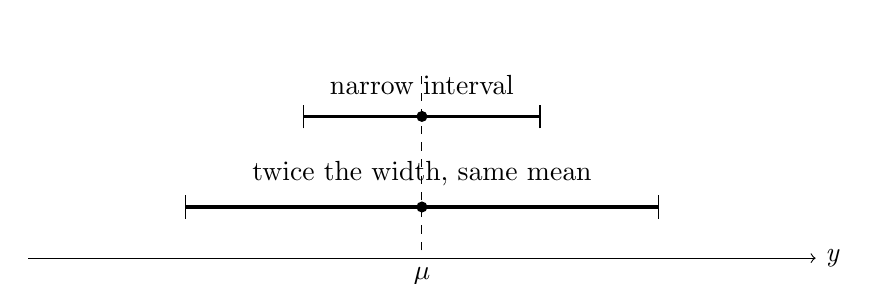
\begin{tikzpicture}[x=1cm,y=1cm]
\draw[->] (0,0)--(10,0) node[right] {$y$};
\draw[dashed] (5,.1)--(5,2.4);
\draw[very thick] (3.5,1.8)--(6.5,1.8);\fill (5,1.8) circle(2pt);
\draw (3.5,1.65)--(3.5,1.95);\draw (6.5,1.65)--(6.5,1.95);
\node[above] at (5,1.95) {narrow interval};
\draw[very thick] (2,.65)--(8,.65);\fill (5,.65) circle(2pt);
\draw (2,.5)--(2,.8);\draw (8,.5)--(8,.8);
\node[above] at (5,.8) {twice the width, same mean};
\node[below] at (5,0) {$\mu$};
\end{tikzpicture}
\end{center}
\textbf{Prediction question.} Which model would you trust near an operating
limit? Width alone cannot answer: inspect accuracy, coverage and the physical
mechanisms omitted from the model.

\section{What Week 2.1 adds to supervised learning}
Week 2 introduced features and targets, scaling, loss functions and complete-case
splits. Here the model additionally states an observation process, computes a
posterior predictive distribution, scores that distribution and calibrates its
width without consulting test cases. No new neural architecture is required.
The first worked example is exact linear Gaussian inference. This lets us
separate probability assumptions from the optimization difficulties of a large
network. The later field example combines a POD representation with Gaussian
processes for its coefficients.

By the end, you should be able to explain what is random, compute a scalar
posterior by hand, identify the terms in predictive variance, distinguish a
marginal interval from a whole-field guarantee, and report a failed coverage
target honestly. Running a plotting cell alone does not demonstrate these skills.

\section{Three sources of uncertainty}
\begin{description}
\item[Aleatoric uncertainty] describes variability such as measurement noise
or unresolved fluctuations. More observations do not necessarily remove the
variability of the next observation, though they may estimate its distribution
more accurately.
\item[Epistemic uncertainty] describes incomplete knowledge of the map or its
parameters. Informative new cases can reduce this component within the model's
assumptions. Repeated optimizer seeds measure only one restricted source of
variation; their spread is not automatically the entire epistemic uncertainty.
\item[Simulator discrepancy] describes the difference between the simulator
and physical reality, including missing physics and numerical limitations.
A surrogate can confidently reproduce a biased CFD solver. A posterior over
surrogate coefficients alone does not include this discrepancy.
\end{description}
Do not combine these mechanisms into an unexplained error bar. For every
reported interval, write what random experiment or uncertainty source it covers.
In particular, noise added to a retained CFD field is an artificial observation
experiment, not an independent new CFD realization.

\section{A Gaussian likelihood and its complete loss}
Suppose independent observations satisfy
\[
y_i=f_\theta(x_i)+\epsilon_i,\qquad \epsilon_i\sim\mathcal N(0,\sigma^2).
\]
The likelihood is a product of Gaussian densities. Taking its negative logarithm gives
\[
-\log p(\mathbf y\mid\theta,\sigma^2)
=\frac n2\log(2\pi)+n\log\sigma+
\frac{1}{2\sigma^2}\sum_{i=1}^n[y_i-f_\theta(x_i)]^2.
\]
If $\sigma$ is known and fixed, minimizing this expression with respect to
$\theta$ is equivalent to minimizing MSE. This is one probabilistic
interpretation of squared-error fitting, not a proof that all physical errors
are Gaussian. If $\sigma$ is learned, $n\log\sigma$ is essential. Omitting it
would reward making the variance arbitrarily large. With varying local noise,
a heteroscedastic model needs a separate variance and logarithmic penalty for
each observation, along with constraints that keep every variance positive.

\begin{worked}{Numerical likelihood check}
For one observation with $y=\mu$, the NLL values for $\sigma=.5,1,2$ are
approximately $.2258,.9189,1.6121$. If instead $y-\mu=1$, they become
$2.2258,1.4189,1.7371$. The very narrow model is penalized when it confidently
misses the observation. The Gaussian density and NLL depend on the units of
$y$; compare scores under the same normalization and state those units.
\end{worked}

\section{Bayesian linear regression as an exact update}
For the linear model $\mathbf y=\Phi\mathbf w+\boldsymbol\epsilon$, let
$\mathbf w\sim\mathcal N(\mathbf m_0,S_0)$ and
$\boldsymbol\epsilon\sim\mathcal N(0,\sigma^2I)$, independently. If there
are $n$ observations and $d$ coefficients, $\Phi$ is $n\times d$,
$\mathbf w$ is $d\times1$ and $S_0$ is $d\times d$.
Bayes' rule multiplies prior and likelihood. Expanding their quadratic forms
and collecting terms in $\mathbf w$ gives
\begin{align*}
S_n^{-1}&=S_0^{-1}+\sigma^{-2}\Phi^T\Phi,\\
\mathbf m_n&=S_n(S_0^{-1}\mathbf m_0+\sigma^{-2}\Phi^T\mathbf y),\\
\mathbf w\mid\mathbf y&\sim\mathcal N(\mathbf m_n,S_n).
\end{align*}
Posterior precision equals prior precision plus data precision. This expression
also identifies why directions poorly excited by $\Phi$ remain uncertain.
Use linear solves or a factorization in code rather than explicitly inverting
large matrices. All covariance matrices must be symmetric and physically and
numerically consistent with their declared units.

\begin{worked}{Poiseuille amplitude with two observations}
Write a normalized parabolic velocity field as $u(y)=w\phi(y)$, where the
known shape $\phi$ is fixed and the unknown scalar amplitude has prior
$w\sim\mathcal N(1,.25^2)$. For a simple hand calculation, use two normalized
measurements with unit basis values: $\Phi=(1,1)^T$, observations $(.9,1.1)^T$
and known $\sigma=.1$. Then
\[
S_n^{-1}=16+200=216,\qquad m_n=(16+90+110)/216=1,
\quad S_n=1/216.
\]
The notebook uses the same principle with a larger sensor set; its result is
not a nonlinear turbulence-model inference. As an exercise, discard the second
measurement. The posterior precision is $116$, mean $106/116=.913793$ and
variance $1/116$. Less data increase parameter uncertainty but do not change
the declared variance of the next measurement's noise.
\end{worked}

\section{Predictive uncertainty has two terms}
For a new basis vector $\phi_*$, the latent prediction $f_* =\phi_*^T\mathbf w$
has mean $\phi_*^T\mathbf m_n$ and variance $\phi_*^TS_n\phi_*$. A noisy
future observation adds a separate noise term:
\[
\operatorname{Var}(y_*\mid x_*,\mathcal D)
=\underbrace{\sigma^2}_{\text{observation noise}}
+\underbrace{\phi_*^TS_n\phi_*}_{\text{parameter uncertainty}}.
\]
For the two-measurement example with $\phi_*=1$, latent variance is
$.00462963$ and predictive observation variance is $.01462963$. The Gaussian
95\% predictive interval is approximately $1\pm .2371$. The latent interval is
narrower. Neither interval includes simulator discrepancy unless a separate
model for it has been added. If $\phi_*=0$ at a prescribed boundary, coefficient
uncertainty contributes zero there; that does not prove all physical boundary
uncertainty is zero.

\textbf{Checkpoint.} State whether a plotted band is for latent velocity,
noisy observation, a pointwise quantity, or an entire field. Explain what changes
when observations are correlated. Replacing a diagonal noise covariance with
a full matrix changes the precision update; counting correlated samples as
independent can produce unjustified confidence.

\newpage
\part*{Part B: field uncertainty after the POD prerequisite}
\addcontentsline{toc}{part}{Part B: field uncertainty after the POD prerequisite}
\section{POD compresses field uncertainty}
Arrange complete training fields into snapshot rows, subtract the training mean
and compute an SVD. Retain $r$ spatial modes in $\Phi_r$:
\[
\mathbf u(Re)\approx\overline{\mathbf u}+\Phi_r\mathbf a(Re).
\]
The input Reynolds number is a case parameter, and the coefficients are functions
of that parameter. A GP for each retained coefficient predicts a distribution
rather than a single coefficient. A fixed low-rank basis reduces a large field
problem to a small number of probabilistic regression problems. It does not
make omitted modes disappear from the physical error.

For training coefficient values $\mathbf a$ with zero prior mean, covariance
matrix $K$ and noise variance $\tau^2$, a test cross-covariance vector $k_*$ and
prior variance $k_{**}$ give
\begin{align*}
\mu_* &= k_*^T(K+\tau^2I)^{-1}\mathbf a,\\
s_*^2 &= k_{**}-k_*^T(K+\tau^2I)^{-1}k_*.
\end{align*}
The second expression is latent variance. Add $\tau^2$ when predicting a noisy
coefficient observation under that model. Kernel amplitude has coefficient-squared
units; length scale has input units. Scaling the input changes the numerical
meaning of a length scale, so report both normalization and kernel settings.

\begin{worked}{A two-observation GP, computed by hand}
Let $K=\left[\begin{smallmatrix}1&.5\\.5&1\end{smallmatrix}\right]$,
$\tau^2=.25$, observations $(1,-1)^T$, $k_*=(.5,.5)^T$ and $k_{**}=1$.
Solving $(K+.25I)\alpha=\mathbf a$ gives
$\alpha=(4/3,-4/3)^T$, hence $\mu_*=0$.
Solving the same matrix against $k_*$ gives $(2/7,2/7)^T$, so
$s_*^2=1-2/7=5/7$. Observation variance would be $5/7+1/4=27/28$.
Explain why opposite observed coefficients give a zero mean at a symmetric
query while leaving nonzero uncertainty.
\end{worked}
Field covariance propagates as
$\operatorname{Cov}(\mathbf u_*)=\Phi_r\operatorname{Cov}(\mathbf a_*)\Phi_r^T$.
Independent coefficient GPs omit cross-coefficient posterior dependence;
retaining only a field covariance diagonal also omits spatial correlation.
Pointwise marginal intervals therefore do not constitute a simultaneous
whole-field coverage guarantee. Truncation error, CFD discretization error and
model discrepancy remain additional limitations.

\section{Calibration stops before the test gate}
The retained author protocol used development cases
$Re=100,150,200,225,250,350,400$, a calibration case $Re=300$,
and held-out cases $Re=175,275,375$. Fit the mean/basis/kernel only with their
permitted development data. Use the calibration case to select an interval
scale, then freeze it. The statistical split unit is a complete Reynolds case,
not random grid nodes from the same field.

A constant multiplier on standard deviation can repair a scale mismatch on
validation. It cannot repair every missing physical mechanism, a wrongly shaped
uncertainty field or distribution shift. A single calibration case also gives
limited evidence about transfer across parameter space. Record the candidates,
criterion, selected scale and time of freezing before opening the test table.

\begin{worked}{Public reuse and truly untouched assessment}
The retained test fields are now visible in the course and in earlier lessons.
Their exclusion from fitting remains meaningful, but they are public held-out
regression cases for a continuing student. A new blind student claim requires
new instructor-held fields revealed only after a frozen protocol. Otherwise
report a reproducible public-case study. Later diagnostic changes motivated by
observing test failures are post-hoc analyses, not repairs validated on that same
untouched test. The notebook labels its later diagnostic extension accordingly.
\end{worked}

\section{Accuracy, calibration and sharpness}
Accuracy asks whether predictive mass lies near truth. Calibration asks whether
nominal levels match empirical frequencies in the declared evaluation setting.
Sharpness asks whether intervals are as narrow as justified. Optimizing only one
can produce an unhelpful distribution. A very wide interval may cover nearly
all observations but provide little discrimination; a narrow interval may miss
confidently. Report all three rather than a single attractive band.

For a nominal central Gaussian level $1-\alpha$, the marginal interval is
$[\mu-z_{1-\alpha/2}s,\mu+z_{1-\alpha/2}s]$. Empirical pointwise coverage is
the fraction of evaluated values falling within their corresponding interval.
Report nominal level, actual coverage, mean width and case count. Grid nodes
share a flow field and are strongly dependent, so their number must not be
presented as the number of independent CFD experiments. Casewise summaries
and new complete cases strengthen the interpretation.

\section{Proper scores for the predictive distribution}
For a scalar Gaussian prediction, the negative log likelihood is
\[
\mathrm{NLL}=\tfrac12\log(2\pi s^2)+\frac{(y-\mu)^2}{2s^2}.
\]
A very small $s$ with a wrong mean receives a severe penalty. Ensure the variance
is positive and explain any numerical floor; it is not a fitted physical noise
model. The continuous ranked probability score compares the predictive CDF
$F$ with the observed step CDF:
\[
\mathrm{CRPS}(F,y)=\int_{-\infty}^{\infty}
\bigl[F(z)-\mathbf1\{y\le z\}\bigr]^2\,dz.
\]
Lower scores are better under the same target definition and units. CRPS has
the units of the target. For a Gaussian with $y=\mu$,
$\mathrm{CRPS}=s(\sqrt2-1)/\sqrt\pi\simeq .233695s$.
The likelihood example in Part A shows why confident errors matter. Apply both
scores to the same cases and pair them with coverage and width. Do not use
pointwise scores to silently claim joint distribution calibration.

\section{Reading the retained field evidence}
The original figure compares the CFD speed field, POD--GP mean speed, vector
error and calibrated marginal spread at $Re=275$, together with coverage
curves. The figure on the following full-width evidence page is enlarged without changing
its pixels or underlying data. It is retained author evidence, not a rerun.
Read the error and spread panels separately: a visually plausible uncertainty
pattern is not a demonstrated probability statement.

The retained mean POD--GP relative $L_2$ error is $0.333\%$, compared with
$0.414\%$ for mean interpolation. At nominal 90\%, the calibrated pointwise
coverage is $65.2\%$. The mean improved while coverage remained substantially
below the target. Validation-only rescaling increased coverage but did not
establish calibration across the held-out Reynolds cases. Preserve this failure
in the report; it teaches more than changing the interval until the displayed
case looks successful.

\clearpage
\thispagestyle{plain}
\begin{center}
{\Large\bfseries Retained CFD uncertainty evidence}\par\vspace{8mm}
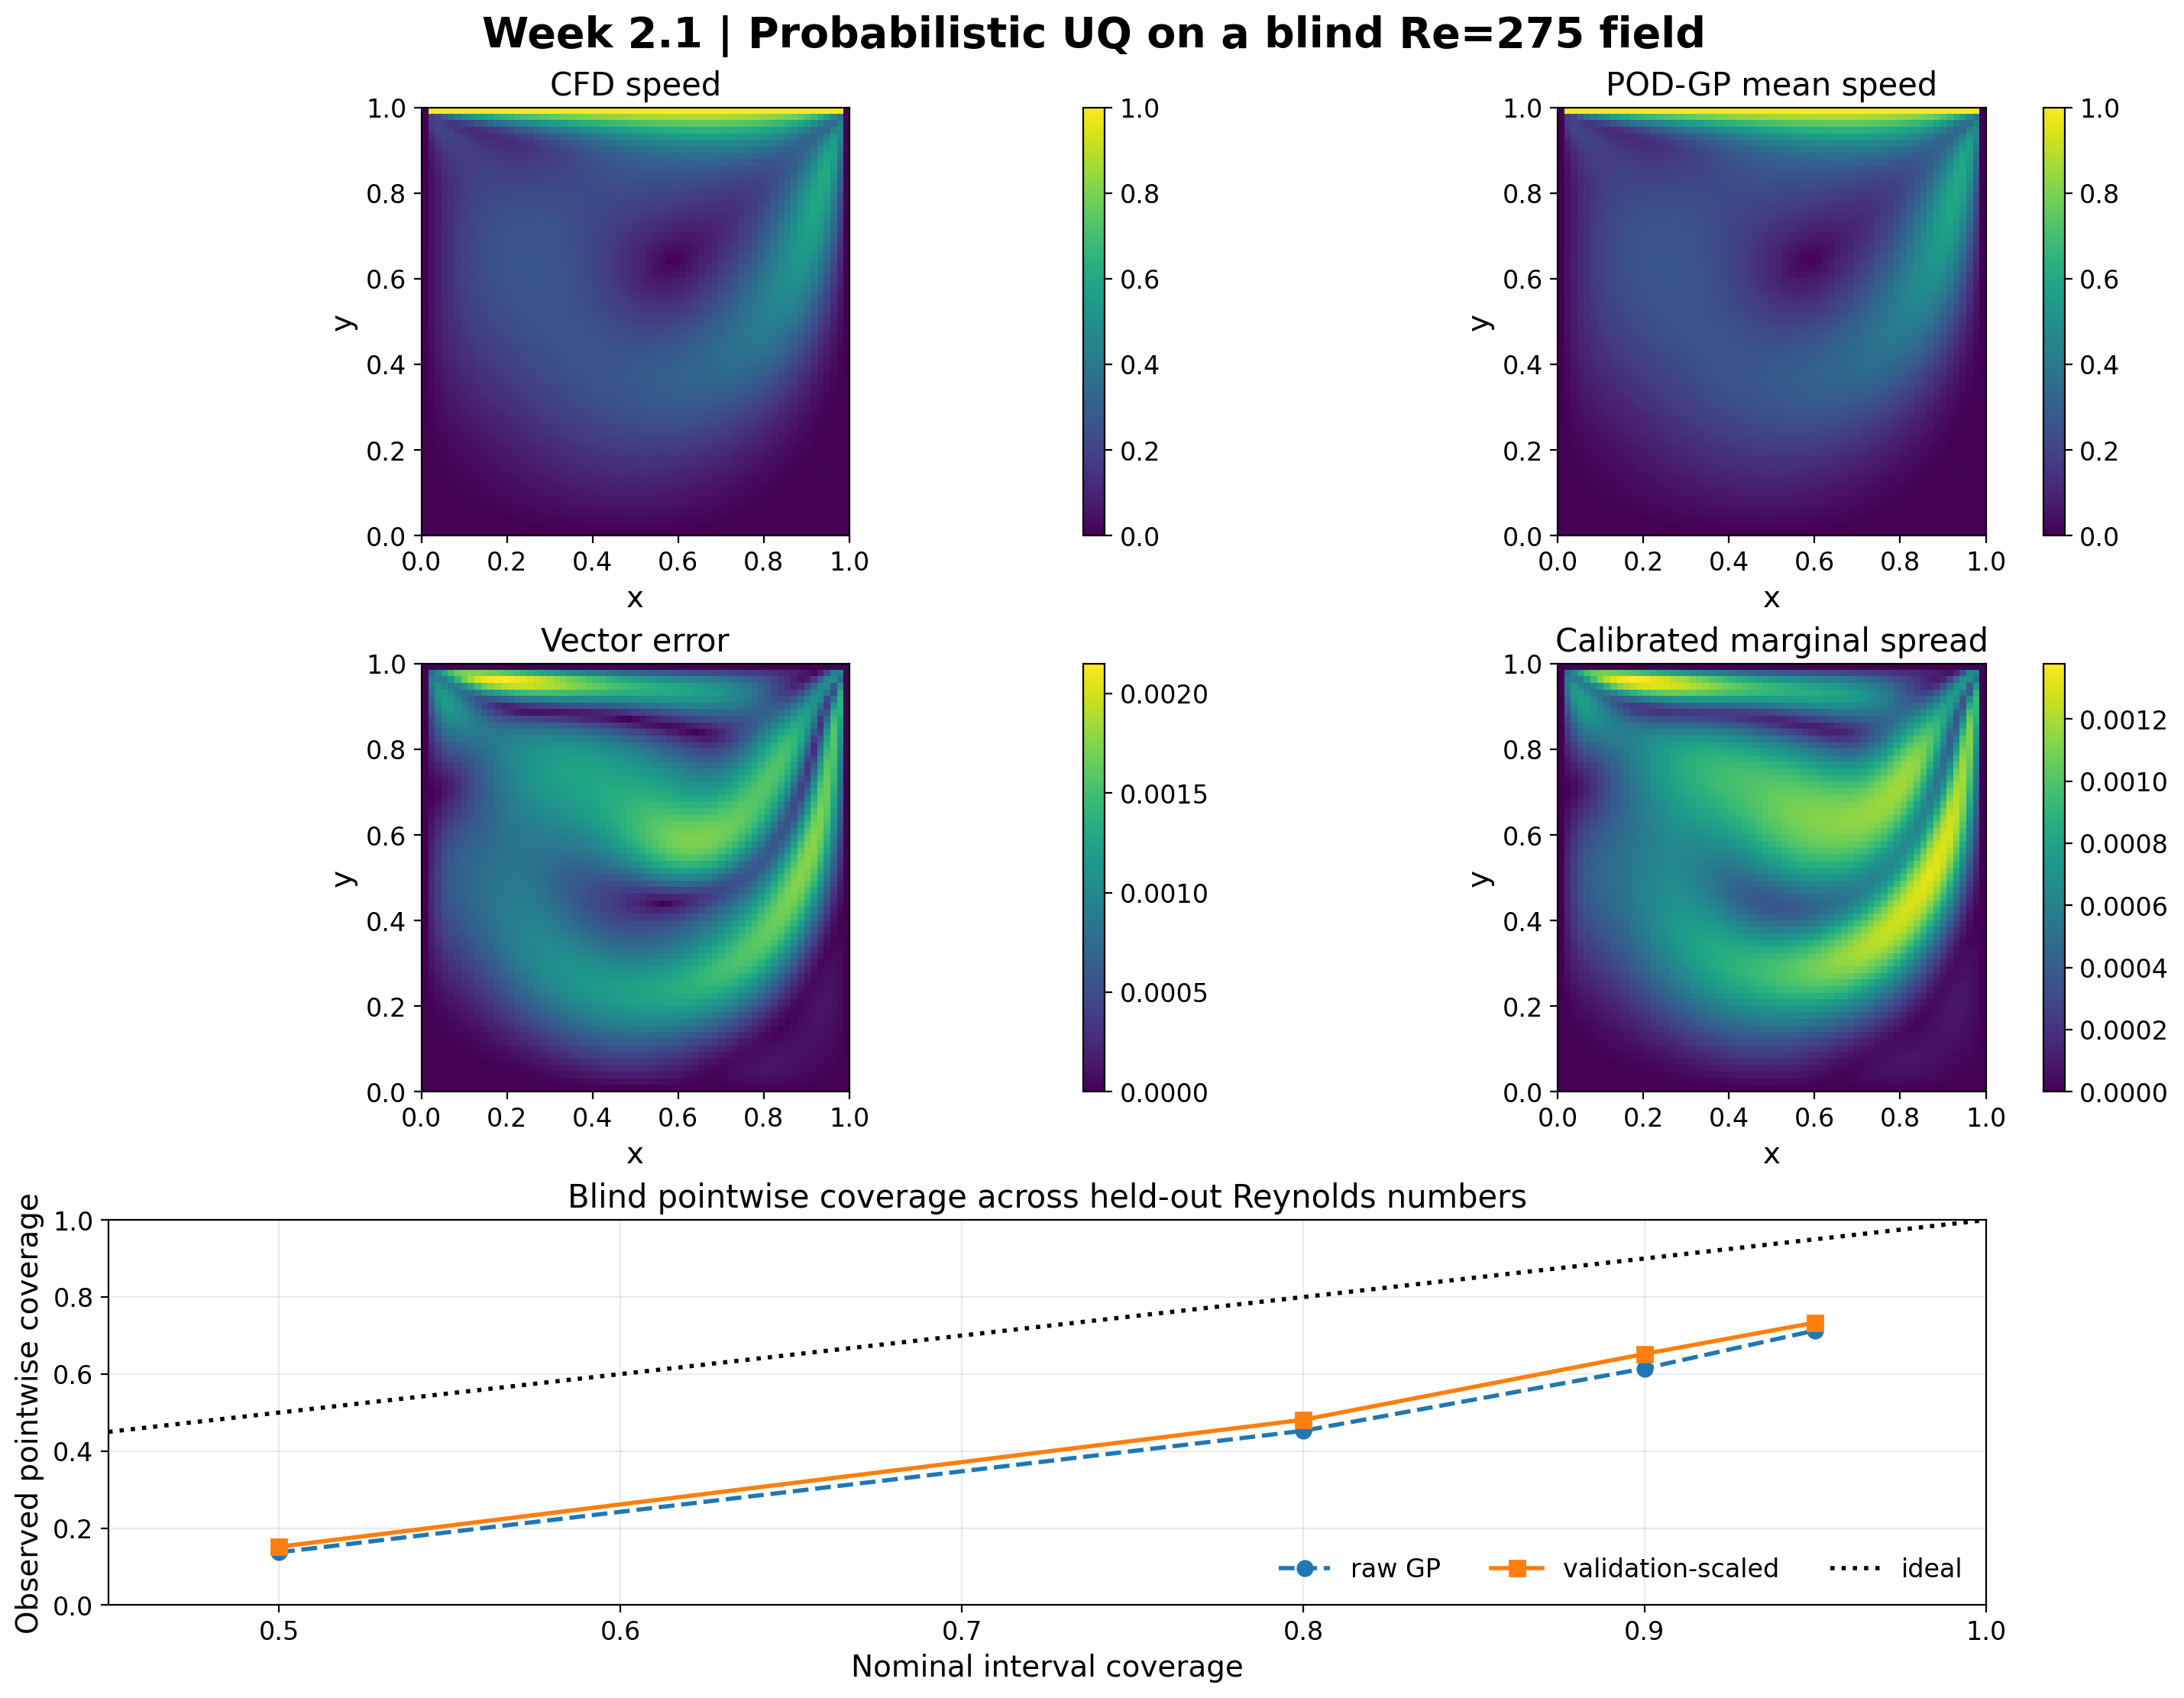
\includegraphics[width=.98\linewidth,height=190mm,keepaspectratio]{results/probabilistic_uq/probabilistic_uq_validation.png}
\end{center}
\noindent Original field panels: held-out $Re=275$ under the author protocol.
Raster scientific evidence is preserved. The searchable equations and exact
metric interpretation appear in the surrounding text. Image provenance:
\texttt{results/probabilistic\_uq/}; no solver or fitting run was performed for
this re-layout.
\clearpage

\section{An uncertainty conclusion with appropriate limits}
A defensible conclusion distinguishes mean accuracy from uncertainty reliability:
within the retained cavity family, the tested POD--GP mean improves on the
specified interpolation comparator, while its nominal 90\% marginal intervals
remain under-covering. This does not establish model-discrepancy calibration,
whole-field coverage or extrapolation safety. Potential future studies include
additional independent calibration cases, explicit discrepancy modelling and
checks of omitted modal/cross-coefficient covariance. These are proposals,
not outcomes demonstrated by the existing figure.

\begin{worked}{Worked interpretation question}
A surrogate has lower relative field error but only 65.2\% empirical coverage at
nominal 90\%. Should it be called a calibrated 90\% predictor? No. Report its
improved mean and failed coverage target together. If you change the kernel or
interval rule after seeing this failure, use fresh untouched cases for a final
claim. The old fields may remain a useful diagnostic regression set.
\end{worked}

\section{Exit checklist, exercises and sources}
Before submitting, state what is random and what mechanisms are omitted; list
complete physical cases and prior exposure; freeze calibration before test;
report accuracy, coverage, width, NLL and CRPS; preserve under-coverage as evidence.

\begin{enumerate}
\item Recompute the scalar two-observation posterior and the one-observation
variant without the helper. Give latent and noisy predictive variance separately.
\item Recompute the two-observation GP solve, including matrix dimensions and
units. Show why a kernel covariance must be positive semidefinite.
\item For predictions with the same mean and $s=.5,1,2$, compute NLL at zero and
unit residual. Explain why widening every interval cannot optimize all criteria.
\item Explain why 4225 grid nodes from one CFD case are not 4225 independent
validation cases, and why pointwise coverage is not simultaneous field coverage.
\item Propose new data that would help distinguish sparse-parameter uncertainty
from CFD model discrepancy. Measurements or an independently qualified simulator
address a different question from simply adding more points from one field.
\end{enumerate}

The notebook and retained protocol are the primary sources for the numerical
experiment. For probability and GP derivations, see Rasmussen and Williams,
\emph{Gaussian Processes for Machine Learning},\href{https://gaussianprocess.org/gpml/}{open textbook}.
For proper scoring rules see Gneiting and Raftery (2007),
\href{https://doi.org/10.1198/016214506000001437}{proper scoring rules article}.
For the distinction between parameter uncertainty and model discrepancy, see
Kennedy and O'Hagan (2001),
\href{https://doi.org/10.1111/1467-9868.00294}{model discrepancy article}.
These references support the concepts; they do not independently validate the
course CFD labels or the retained coverage experiment.
\end{document}
